% -*- TeX:UTF-8 -*-
%%
%% KAIST 학위논문양식 LaTeX용 (ver 0.5) 예시
%%
%% @version 0.4
%% @author  채승병 Chae,Seungbyung (mailto:chess@kaist.ac.kr)
%% @date    2004. 11. 12.
%%
%% @requirement
%% teTeX, fpTeX, teTeX 등의 LaTeX2e 배포판
%% + 은광희 님의 HLaTeX 0.991 이상 버젼 또는 홍석호 님의 HPACK 1.0
%% : 설치에 대한 자세한 정보는 http://www.ktug.or.kr을 참조바랍니다.
%%
%% @note
%% 기존에 널리 쓰여오던 차재춘 님의 학위논문양식 클래스 파일의 형식을
%% 따르지 않고 전면적으로 다시 작성하였습니다. 논문 정보 입력부분에서
%% 과거 양식과 다른 부분이 많으니 아래 예시에 맞춰 바꿔주십시오.
%%
%%
%% @acknowledgement
%% 본 예시 논문은 물리학과 박사과정 김용현 님의 호의로 제공되었습니다.
%%
%% -------------------------------------------------------------------
%% @information
%% 이 예제 파일은 hangul-ucs를 사용합니다. UTF-8 입력 인코딩으로
%% 작성되었습니다. hlatex의 hfont는 이용하지 않습니다. --2006/02/11
%% 본 템플릿은 전산학부 김민혁 교수에의해서 버그 수정되었습니다. -- 2016/11/25
%% 본 템플릿은 전산학부 김민혁 교수에의해서 추가 버그 수정되었습니다. -- 2023/06/15

% @class kaist.cls
% @options [default: doctor, korean, final]
% - doctor: 박사과정 | master : 석사과정
% - korean: 한글논문 | english: 영문논문
% - final : 최종판   | draft  : 시험판
% - pdfdoc : 선택하지 않으면 북마크와 colorlink를 만들지 않습니다.


% TODO: This is a draft
\documentclass[master,english,draft]{kaist-ucs} % 석사과정
%\documentclass[doctor,english,final]{kaist-ucs} % 박사과정


% If you want make pdf document (include bookmark, colorlink)
%\documentclass[doctor,english,final,pdfdoc]{kaist-ucs}

% kaist.cls 에서는 기본으로 dhucs, ifpdf, graphicx 패키지가 로드됩니다.
% 추가로 필요한 패키지가 있다면 주석을 풀고 적어넣으십시오,
%\usepackage{...}
\usepackage{amsmath}
\usepackage{amssymb}

\allowdisplaybreaks

\newcommand{\red}[1]{\textcolor{red}{#1}}


% @command title 논문 제목(title of thesis)
% @options [default: (none)]
% - korean: 한글제목(korean title) | english: 영문제목(english title)
% TODO: Below is working titles
\title[korean] {AL 의미 수식화 및 AL 타입 시스템 도입}
\title[english]{AL Semantics Formalization and AL Type System Introduction}

% @note 표지에 출력되는 제목을 강제로 줄바꿈하려면 \linebreak 을 삽입.
%       \\ 나 \newline 등을 사용하면 안됩니다. (아래는 예시)
%
%\title[korean]{탄소 나노튜브의 물리적 특성에 대한\linebreak 이론 연구}
%\title[english]{Theoretical study on physical properties of\linebreak
%                carbon nanotubes}
%
% If you want to begin a new line in cover, use \linebreak .
% See examples above.
%


% @command author 저자 이름
% @param   family_name, given_name 성, 이름을 구분해서 입력
% @options [default: (none)]
% - korean: 한글이름 | chinese: 한문이름 | english: 영문이름
% 한문 이름이 없다면 빈 칸으로 두셔도 됩니다.
%
%
% If you are a foreigner , write your name in korean or your korean name.
% If you can't write native character, you can make the chinese blank empty 
% Write as follow
% \author[korean]{family name in korean}{given name in korean}
% \author[chinese]{family name in your native language}{given name in your native language}
% \author[english]{family name in english}{given name in english}
%
\author[korean] {신}{원 호}
\author[korean2] {신}{원호}    %이름을 붙여 써 주시기 바랍니다.
\author[chinese]{申}{元 鎬}
\author[english]{Shin}{Wonho}

% @command advisor 지도교수 이름 (복수가능)
% @usage   \advisor[options]{...한글이름...}{...영문이름...}{signed|nosign}
% @options [default: major]
% - major: 주 지도교수  | coopr: 공동 지도교수
% TODO: sign
\advisor[major]{류 석 영}{Sukyoung Ryu}{nosign}
\advisor[major2]{류석영}{Sukyoung Ryu}{nosign}    %한글 성과 한글 이름을 모두 붙여 써 주시기 바랍니다.

% [주의] 전산학부의 경우, 전공이름(Computer Science)을 적어주시기 바랍니다. 조직명(School of Computing) 적지 말아주세요!
\advisorinfo{Professor of Computer Science} %제출승인서에 들어가는 교수님 정보, advisor's information 

%\advisor[coopr]{홍 길 동}{Gil-Dong Hong}{nosign}
%\advisor[coopr2]{홍길동}{Gil-Dong Hong}{nosign}    %한글 성과 한글 이름을 모두 붙여 써 주시기 바랍니다.
%
% 지도교수 한글이름은 입력하지 않아도 됩니다.
% You may not input advisor's korean name
% like this \advisor[major]{}{Chang, Kee Joo}{signed}
%


% @command department {학과이름}{학위종류} - 아래 규칙에 따라 코드를 입력
% @command department {department code}{degree field}
%
% department code
% 2. 석박사학위논문 작성 및 제출요령 4쪽 ~ 5쪽 참고
% 또는 kaist-ucs.cls 의 % @command department 참고

% science: 이학 | engineering: 공학 | business : 경영학
% 박사논문의 경우는 학위종류를 입력하지 않아도 됩니다.
% If you write Ph.D. dissertation, you cannot input degree field.
% The third parameter : a | b | c
% a: 소속된 학과만 쓰는 옵션 (학과에만 소속되어 있는 경우에는 무조건 a를 선택해야 함)
% b: 학과 아래의, 프로그램이나 학제전공에 소속되어 있을 경우에 학과와 프로그램을 함께 쓰는 옵션
% c: 학과 아래의, 프로그램이나 학제전공에 소속되어 있을 경우에 학과를 쓰지 않고 프로그램이나 학제전공의 이름만 쓰는 옵션 
% 
% a: it represents only the name of department. (if you aren't in the program under the department, must choose a)
% b: it represents the names of department and the program that is under the department (consider this when you are in the program not only department)
% c: it represents only the name of program that is under the department (consider this when you are in the program not only department)
\department{CS}{engineering}{a}

% @command referee 심사위원 (석사과정 3인, 박사과정 5인)
\referee[1]{류 석 영}
\referee[2]{유 신}
\referee[3]{허 기 홍}
% Of course english name is available

% @command approvaldate 지도교수논문승인일
% @param   year,month,day 연,월,일 순으로 입력
% TODO: not approved!
\approvaldate{2020}{12}{5}

% @command refereedate 심사위원논문심사일
% @param   year,month,day 연,월,일 순으로 입력
% TODO: TBD
\refereedate{2020}{12}{5}

% @command gradyear 졸업년도
\gradyear{2025}

% 본문 시작
\begin{document}

  % 앞표지, 속표지, 학위논문 제출승인서, 학위논문 심사완료 검인서는
  % 클래스 옵션을 final로 지정해주면 자동으로 생성되며,
  % 반대로 옵션을 draft로 지정해주면 생성되지 않습니다.

  % 논문 서지, 초록, 핵심 낱말, 영문 초록, 영어 핵심 낱말 (Information of thesis, abstract in korean, keywords in korean, abstract in english, keywords in english)
 \thesisinfo
 %% Letters of abstract in korean must be less than 500 and words of abstract in english must be less than 300.
 %% Number of keywords must be less than 6.
 %% Don't write english letters in the abstract in korean.
  \begin{summary}
  % TODO: Korean abstract
  초록초록

  \end{summary}

  \begin{Korkeyword}
  % TODO: Korean keyword
  \end{Korkeyword}


  \begin{abstract}
  % TODO: English abstract
  Greengreen
  \end{abstract}

  \begin{Engkeyword}
  % TODO: English keyword
  \end{Engkeyword}


  \addtocounter{pagemarker}{1}                 % 백색별지분을 고려
  \newpage



  % 목차 (Table of Contents) 생성
  \tableofcontents

  % 표목차 (List of Tables) 생성
  \listoftables

  % 그림목차 (List of Figures) 생성
  \listoffigures

  % 위의 세 종류의 목차는 한꺼번에 다음 명령으로 생성할 수도 있습니다.
  %\makecontents

%% 이하의 본문은 LaTeX 표준 클래스 report 양식에 준하여 작성하시면 됩니다.
%% 하지만 part는 사용하지 못하도록 제거하였으므로, chapter가 문서 내의
%% 최상위 분류 단위가 됩니다.
%% You cannot use 'part'

% !TEX root = main.tex

\chapter{Introduction}
\label{ch:intro}
\noindent

\begin{itemize}
\item Wasm
  \begin{itemize}
  \item is low-level bytecode language, platform-indep, ...
  \item is compile target for Web applications
  \item is used in wide area such as IoT, ...
  \end{itemize}
\item Wasm Spec
  \begin{itemize}
  \item descibes syntax and semantics of Wasm
  \item should be rigorous because ... (brief explanation for two format)
  \item has two format to describe semantics (formal\&prose notation)
  \item formal notation is written in math expression: concise, clear, amenable to proofs, ...
  \item prose notation is step by step instruction written English: vague (in some part), amenable to developing engines
  \end{itemize}
\item SpecTec
  \begin{itemize}
  \item is proposed to alleviate spec writing process
  \item is accepted by Wasm committee to be an official Wasm specification tool
  \item define AL to describe Wasm semantics in prose notation
  \item AL is designed to be similar to prose notation (describe with fig)
  \item implement AL interpreter to make the spec executable
  \item executable spec passes official wasm test $\leftarrow$ correctness
  \end{itemize}
\item Problem
  \begin{itemize}
  \item no semantics in AL
  \item prose notation is still vague unless read AL interpreter code
  \item ???
  \end{itemize}
\item Contribution
  \begin{itemize}
  \item formalize AL syntax$\&$semantics
  \item make prose notation clear to understand
  \item ???
  \end{itemize}
\end{itemize}


% breif overview
WebAssembly (Wasm)~\cite{wasm} is a low-level bytecode language that is safe, fast,
portable, and compact.
It is widely used as a compilation target for web applications.
Beyond web development, Wasm's advantages are also deployed in areas such as
edge computing~\cite{wasm-edge}, IoT~\cite{wasm-iot}, and
blockchain~\cite{wasm-block}.


% risk of implementation divergence
There are numerous Wasm engines, with all major browsers implementing their own
multi-tiered versions~\cite{v8, spidermonkey, webkit}.
Additionally, specialized engines target specific domains, such as embedded
systems and edge computing.
However, ensuring portability across these diverse implementations introduces
the risk of divergence among them.


% rigorous standardization -> spec is rigorous: formal notation & prose notation
To address this challenge, Wasm has been rigorously standardized by the
W3C~\cite{wasm-w3c}.
The Wasm specification is particularly rigorous, describing its semantics in
two complementary forms: formal notation and prose notation.
The formal notation employs mathematical rules to succinctly define the
semantics, supporting proofs such as type soundness.
Conversely, the prose notation uses pseudocode-like algorithms to explain the
semantics through step-by-step instructions.
Since most Wasm users and engine developers are less familiar with mathematical
formalism, they primarily rely on the prose notation.


% challenging specification process
The demanding standardization process places a significant burden on
specification authors.
Crafting this specification document is labor-intensive, and as Wasm evolves,
the manual effort required becomes increasingly challenging to scale.
Moreover, the dual requirement of maintaining both the formal notation and
prose notation exacerbates these difficulties.
The formal notation is written in LaTeX, and the prose notation is authored
in reStructuredText; neither of which is particularly user-friendly for
collaborative review.
This lack of accessibility in the specification's tooling increases the
likelihood of inconsistensies and errors, further complicating the
standardization effort.


% SpecTec
To alleviate this problem, we had been developing SpecTec, a framework for
mechanizing WebAssembly specification.
It provides DSL to define Wasm syntax and semantics in a declarative style
similar to the formal notation.
It type-checks DSL to prevent meta-level specification errors, and generates
many artifacts including the specification document, a Wasm interpreter, and
mechanized definitions for theorem provers.


% AL
To express 


% problem
However, AL cannot describe Wasm control flow correctly


% contribution
build AL's computation model for Wasm, formalize AL semantics


% !TEX root = main.tex

\chapter{Background}
\label{ch:background}
\noindent


\section{WebAssembly}

% breif overview
WebAssembly is a low-level bytecode language that is safe, fast, portable, and
compact~\cite{wasm}.
It is widely used as a compile target for web applications.
Furthermore, many areas other than Web such as edge computing~\cite{wasm-edge},
IoT~\cite{wasm-iot}, and block chains~\cite{wasm-block} deploy the advantages
of WebAssembly.

% risk of implementation divergence
There are dozens of WebAssembly engines; all the browsers have there own
implementations of WebAssembly with multiple tiers, and there are many engines
that target for specific areas including embedded systems and edge computing.
As a consequence, implementations of WebAssembly could diverge.

% rigorous standardization -> formal notation & prose notation
To handle this problem, WebAssembly has been standardized very rigourously by
the W3C~\cite{wasm-w3c}.
One of the requirements to standardize a feature is to describe the semantics
of WebAssembly in two forms: formal notation and prose notation.
Formal notation uses mathematical rules to compactly describe the semantics,
and it is used for proofs such as type soundness.
On the other hand, prose notation uses psudocodes to explain the semantics
step by step.
People such as WebAssembly engine developers who are not familiar with
mathematical rules utilize it.

% structure: module, function, ...

% execution: instantiation, invocation, ...

% control structure: label frame block ...


\section{SpecTec}


% !TEX root = main.tex

\chapter{Motivation}
\label{ch:motivation}
\noindent

\newcommand{\officialp}{official prose}
\newcommand{\spectecp}{SpecTec prose}

\red{TODO: remove redundant part in the fig}



% control flow structure in official prose
It might be easy to understand how the \officialp{} explains the control flow
of WebAssembly, if we assume that a WebAssembly code is loaded on a memory and
a pc points to the instruction to execute.
To describe control flow, it uses a structure named \textit{block} which
consitutes of a instruction sequence.
When executing the instructions in the block, pc can be changed to the starting
point of the block or the end of the block.


% an example of Wasm control flow
\textbf{Example 1}
\begin{verbatim}
  // infinite loop
  (loop (result i32) (i32.const 42) (br 0) (unreachable) end) (unreachable)
\end{verbatim}

Example 1 is a WebAssembly code example that has \texttt{loop} and
\texttt{unreachable}
Here, result type of the \texttt{loop} is \texttt{i32} and the \texttt{loop}
has a block of three instructions: \texttt{i32.const}, \texttt{br}, and
\texttt{unreachable}.
\cref{fig:loop} is the \officialp{} of the \texttt{loop} instruction.
It says that the continuation is the start of the loop, the information is
stored in a label, and it \textit{enters} the block with the label.
The term \textit{enter} means that it pushes the label in the stack and makes
pc points to the first instruction in the block.
The \texttt{i32.const} instruction is executed first, which just pushes the
\texttt{i32} value \texttt{42} in the stack.
Then, The \texttt{br} instruction is executed.
\cref{fig:br} is the \officialp{} of the \texttt{br} instruction.
It pops the label from the stack, and makes pc points to the continuation of
the label, which is the start of the loop instruction.
As a result, the code example above is a infinite loop pushing \texttt{42}
forever without executing \texttt{unreachable} instruction.

\begin{figure}[h!]
    \centerline{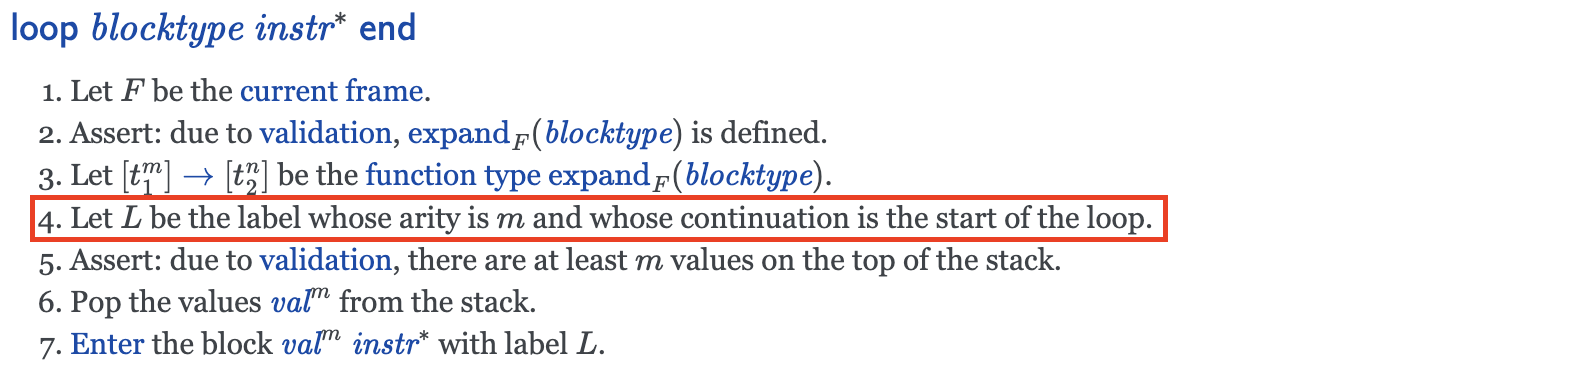
\includegraphics[width=15cm]{fig/loop}}
    \caption[Enter the caption title here]{\texttt{loop} instruction} \label{fig:loop}
    \centerline{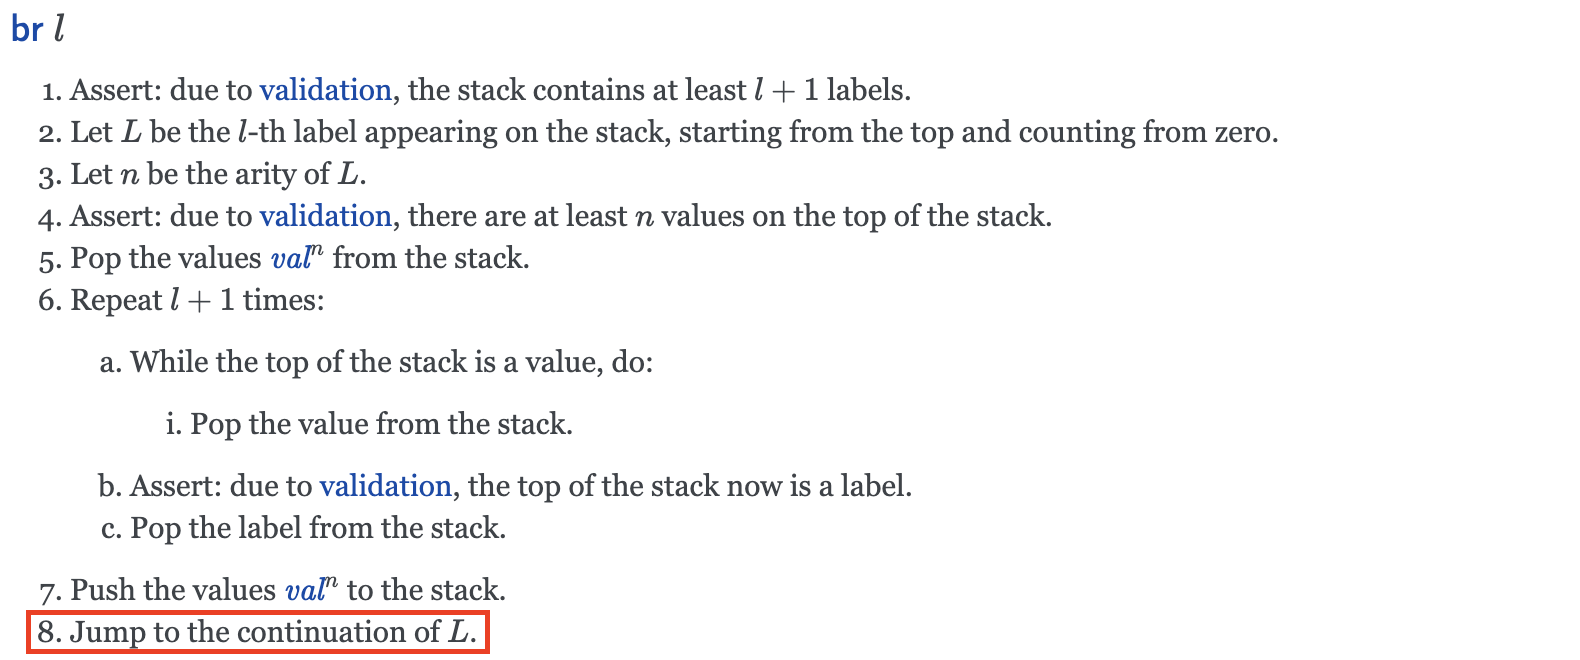
\includegraphics[width=15cm]{fig/br}}
    \caption[Enter the caption title here]{\texttt{br} instruction} \label{fig:br}
\end{figure}


% exit label in official prose
There is also a special form of a behavior related to the block: an
\textit{exit label}.
\cref{fig:exit-label} is the \officialp of the exit label.
It is special because this behavior is not performed without an explicit
WebAssembly instruction.
Rather, the behavior is performed when \textbf{the end of a block is reached}
without control instructions or runtime error.
The behavior is that the label is popped from the stack, and the pc changes to
the point after the end of the block.

\begin{figure}[h!]
    \centerline{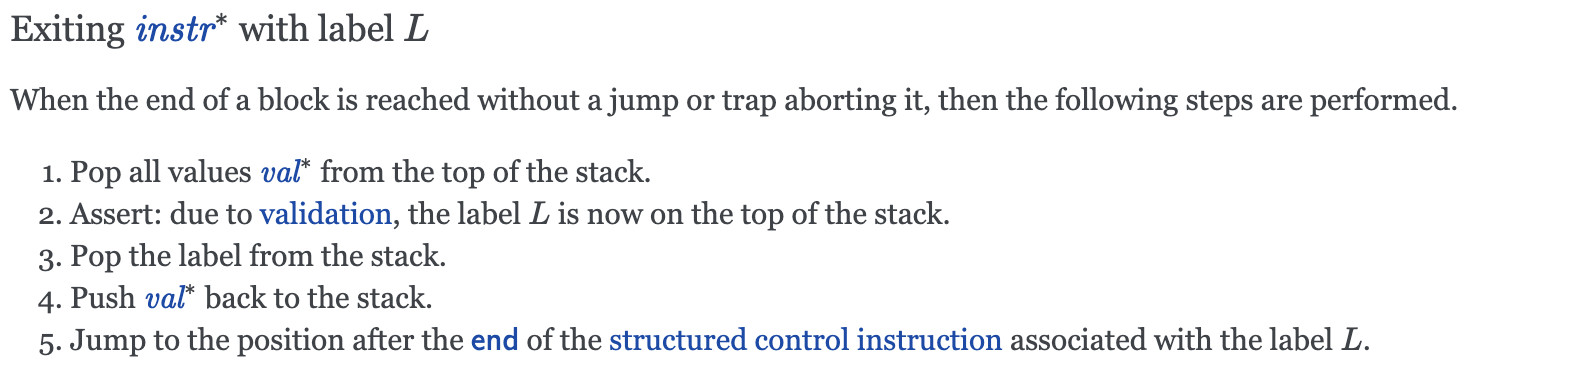
\includegraphics[width=15cm]{fig/exit}}
    \caption[Enter the caption title here]{exit label} \label{fig:exit-label}
\end{figure}


% an example of exit label
\textbf{Example 2}
\begin{verbatim}
  // exit label
  (loop (result i32) (i32.const 42) end) (f64.const 3.14)
\end{verbatim}

Example 2 is \texttt{loop} with a block that has only \texttt{i32.const}.
A label is pushed in the stack when a \texttt{loop} instruction is executed.
After \texttt{i32.const} is executed, the end of the block is reached.
As a result, exit label occurs so that the label is popped from the stack,
pc changes to the point after the end of block: \texttt{f64.const}.
Therefore, the code example above results in the value 42 and 3.14 pushed to
the stack.

Similar to the control flow using the block and the label, there are many other
control instructions and structures such as a \texttt{call} instruction that
calls a function with a frame and a \texttt{return} instruction that returns from
the function with the frame.


TODO: detailed explanation of \spectecp{} w/ fig

However, the \spectecp{} assumes that the \red{machine} takes WebAssembly
instructions one by one, and changes the internal state accordingly without pc.
This is because the \spectecp{} is generated automatically from the \red{dsl}
which uses rewrite rule to describe WebAssembly semantics.
As a result, rather than jump to the start of the loop, \spectecp{} stores the
\texttt{loop} instruction itself in the label, and executes it again if the
\texttt{br} instruction is executed.
Not only that, it doesn't have block structure.

don't remember end!





% official spec prose notation control structure
% seems to be pc-based
% AL from DSL ~ formal notation: no pc
% AL: instruction sequence input continously
% device exit semantics for AL
% Executable spec passes all wasm testcases
% weird, maybe not happened in realworld, but valid wasm code
% wrong!


% !TEX root = main.tex

\chapter{Semantics}
\label{ch:semantics}
\noindent


% AL semantics formalize
%
%
% Prose notation:
% - Implicit when to exit:
%   • Returning from a function
%     When the end of a function is reached without a jump (i.e., return) or trap aborting it, then the following steps are performed.
%
%   • Exiting with label
%     When the end of a block is reached without a jump or trap aborting it, then the following steps are performed.
%
%   ! end of function/label is defined verbally, not in algorithmic notation
%
% - Separate context and instructions:
%   • Push ctx \& Jump instrs
%
%
% abstract machine of prose notation: vm
% 1. state: stack, store
% 2. cosumes sequence of WebAssembly instruction
% 3. mutate state
%
% - store
%   - instantiate -> alloc
%   - invoke -> use
% - stack contains value \& context
%   - value
%     ex: binop
%   - context
%     1) label: allow structured control flow (continuation)
%     2) frame: store call information (local variable, module instance)
%     - enter \& exit
%     - ex: loop, invoke
%     - ex: br, implicit exit
%
%
% - wrong interpretation of "end" in AL interpreter \red{(How long does it occur?)}
% - example

\red{TODO: fix EnterI semantics, change ExitI to PopCtxI}


\newcommand{\sem}[1]{[\![#1]\!]}
\newcommand{\seq}[1]{#1^*}



%% Symbol definition

\renewcommand{\symbol}[1]{\textbf{#1}}

% Continuation
\newcommand{\mt}{\symbol{Empty}}
\newcommand{\call}{\symbol{Call}}
\newcommand{\al}{\symbol{Al}}
\newcommand{\enter}{\symbol{Enter}}
\newcommand{\wasm}{\symbol{Wasm}}
\newcommand{\exe}{\symbol{Execute}}
\newcommand{\ret}{\symbol{Return}}

% Instruction
\newcommand{\ifi}{\symbol{IfI}}
\newcommand{\eitheri}{\symbol{EitherI}}
\newcommand{\enteri}{\symbol{EnterI}}
\newcommand{\pushctxi}{\symbol{PushCtxI}}
\newcommand{\pushi}{\symbol{PushI}}
\newcommand{\popctxi}{\symbol{PopCtxI}}
\newcommand{\popi}{\symbol{PopI}}
\newcommand{\popni}{\symbol{PopNI}}
\newcommand{\popalli}{\symbol{PopAllI}}
\newcommand{\leti}{\symbol{LetI}}
\newcommand{\trapi}{\symbol{TrapI}}
\newcommand{\nopi}{\symbol{NopI}}
\newcommand{\returnrulei}{\symbol{ReturnRuleI}}
\newcommand{\returnfunci}{\symbol{ReturnFuncI}}
\newcommand{\executei}{\symbol{ExecuteI}}
\newcommand{\executeseqi}{\symbol{ExecuteSeqI}}
\newcommand{\performi}{\symbol{PerformI}}
\newcommand{\calli}{\symbol{CallI}}
\newcommand{\replacei}{\symbol{ReplaceI}}

% Expression
\newcommand{\vare}{\symbol{VarE}}
\newcommand{\nume}{\symbol{NumE}}
\newcommand{\boole}{\symbol{BoolE}}
\newcommand{\fnamee}{\symbol{FnameE}}
\newcommand{\une}{\symbol{UnE}}
\newcommand{\bine}{\symbol{BinE}}
\newcommand{\acce}{\symbol{AccE}}
\newcommand{\upde}{\symbol{UpdE}}
\newcommand{\stre}{\symbol{StrE}}
\newcommand{\compe}{\symbol{CompE}}
\newcommand{\cate}{\symbol{CatE}}
\newcommand{\meme}{\symbol{MemE}}
\newcommand{\lene}{\symbol{LenE}}
\newcommand{\tupe}{\symbol{TupE}}
\newcommand{\casee}{\symbol{CaseE}}
\newcommand{\itere}{\symbol{IterE}}
\newcommand{\liste}{\symbol{ListE}}
\newcommand{\getcurctxe}{\symbol{GetCurContextE}}
\newcommand{\choosee}{\symbol{ChooseE}}
\newcommand{\iscaseofe}{\symbol{IsCaseOfE}}
\newcommand{\isvalide}{\symbol{IsValidE}}
\newcommand{\ctxkinde}{\symbol{CtxKindE}}
\newcommand{\matche}{\symbol{MatchE}}
\newcommand{\hastypee}{\symbol{HasTypeE}}

% Unary operator
\newcommand{\notop}{\symbol{NotOp}}
\newcommand{\minusop}{\symbol{MinusOp}}

% Binary operator
\newcommand{\addop}{\symbol{AddOp}}
\newcommand{\subop}{\symbol{SubOp}}
\newcommand{\mulop}{\symbol{MulOp}}
\newcommand{\divop}{\symbol{DivOp}}
\newcommand{\modop}{\symbol{ModOp}}
\newcommand{\expop}{\symbol{ExpOp}}
\newcommand{\implop}{\symbol{ImplOp}}
\newcommand{\equivop}{\symbol{EquivOp}}
\newcommand{\andop}{\symbol{AndOp}}
\newcommand{\orop}{\symbol{OrOp}}
\newcommand{\eqop}{\symbol{EqOp}}
\newcommand{\neop}{\symbol{NeOp}}
\newcommand{\ltop}{\symbol{LtOp}}
\newcommand{\gtop}{\symbol{GtOp}}
\newcommand{\leop}{\symbol{LeOp}}
\newcommand{\geop}{\symbol{GeOp}}

% Path
\newcommand{\idxp}{\symbol{Idx}}
\newcommand{\slicep}{\symbol{Slice}}
\newcommand{\dotp}{\symbol{Dot}}

% Iter
\newcommand{\listiter}{\symbol{List}}
\newcommand{\listniter}{\symbol{ListN}}
\newcommand{\listidxiter}{\symbol{Index}}

% Value
\newcommand{\numv}{\symbol{NumV}}
\newcommand{\boolv}{\symbol{BoolV}}
\newcommand{\listv}{\symbol{ListV}}
\newcommand{\strv}{\symbol{StrV}}
\newcommand{\casev}{\symbol{CaseV}}
\newcommand{\tupv}{\symbol{TupV}}
\newcommand{\fnamev}{\symbol{FnameV}}
\newcommand{\trapv}{\symbol{TrapV}}
\newcommand{\storev}{\symbol{StoreV}}




%% Helper function

\newcommand{\helper}[1]{\text{#1}}

% Helper function
\newcommand{\lookup}{\helper{lookup}}
\newcommand{\execute}{\helper{execute}}
\newcommand{\exit}{\helper{exit}}
\newcommand{\duplicateenv}{\helper{duplicate\_env}}
\newcommand{\getctxcnt}{\helper{get\_ctx\_cnt}}
\newcommand{\increasectxcnt}{\helper{increase\_ctx\_cnt}}
\newcommand{\getenv}{\helper{get\_env}}
\newcommand{\setenv}{\helper{set\_env}}
\newcommand{\prependinstr}{\helper{prepend\_instr}}
\newcommand{\push}{\helper{push}}
\newcommand{\pop}{\helper{pop}}
\newcommand{\popn}{\helper{popn}}
\newcommand{\unop}{\helper{unop}}
\newcommand{\splitctx}{\helper{split\_ctx}}
\newcommand{\getcurctx}{\helper{get\_cur\_ctx}}
\newcommand{\getcurframe}{\helper{get\_cur\_frame}}
\newcommand{\setcurframe}{\helper{set\_cur\_frame}}
\newcommand{\access}{\helper{access}}
\newcommand{\update}{\helper{update}}
\newcommand{\updateidx}{\helper{update\_idx}}
\newcommand{\updateslice}{\helper{update\_slice}}
\newcommand{\updatedot}{\helper{update\_dot}}
\newcommand{\istrue}{\helper{is\_true}}
\newcommand{\isframe}{\helper{is\_frame}}
\newcommand{\zip}{\helper{zip}}
\newcommand{\fold}{\helper{fold}}
% How to express?
\newcommand{\domain}{\helper{domain}}
% Hardcode
\newcommand{\assign}{\helper{assign}}
\newcommand{\iswasmvalueinstr}{\helper{is\_wasm\_value\_instr}}
\newcommand{\binop}{\helper{binop}}
% Reference interpreter
\newcommand{\isvalid}{\helper{is\_valid}}
\newcommand{\match}{\helper{match}}
\newcommand{\hastype}{\helper{has\_type}}




%% Syntax

\begin{align*}
%
% State
  s \in S =& \seq A \times W \times Cont \\
%
% Algorithm
  a \in A =& str \times \seq E \times \seq I \\
%
% Wasm state
  w \in W =& \seq{WasmValue} \times \seq{WasmInstr} \times Store \\
  wv \in WasmValue =& V \\
  wi \in WasmInstr =& V \\
%
% Store
  sto \in Store =& String \mapsto \seq V \\
%
% Continuation
  c \in Cont =& ~ \mt \\
    | & ~ \call ~ String \times \seq V \times Cont \\
    | & ~ \al ~ \seq I \times Env \times \mathbb N \times Cont \\
    | & ~ \wasm ~ \mathbb N \times Cont \\
    | & ~ \exe ~ wi \times Cont \\
    | & ~ \ret ~ V \times Cont \\
%
% Environment
  \mu \in Env =& String \mapsto V \\
%
% Instruction
  i \in I =& ~ \ifi ~ E \times \seq I \times \seq I \\
    | & ~ \eitheri ~ \seq I \times \seq I \\
    | & ~ \enteri ~ E \times E \\
    | & ~ \pushctxi ~ E \\
    | & ~ \pushi ~ E \\
    | & ~ \popctxi ~ E \\
    | & ~ \popi ~ E \\
    | & ~ \popni ~ E \times E \\
    | & ~ \popalli ~ E \\
    | & ~ \leti ~ E \times E \\
    | & ~ \trapi \\
    | & ~ \returnrulei \\
    | & ~ \returnfunci ~ E \\
    | & ~ \executei ~ E \\
    | & ~ \executeseqi ~ E \\
    | & ~ \performi ~ String \times \seq{E} \\
    | & ~ \calli ~ String \times String \times \seq{E} \\
    | & ~ \replacei ~ E \times \seq{Path} \times E \\
%
% Expression
  e \in E =& ~ \vare ~ String \\
    | & ~ \nume ~ \mathbb N \\
    | & ~ \boole ~ \mathbb B \\
    | & ~ \fnamee ~ String \\
    | & ~ \une ~ Unop \times E \\
    | & ~ \bine ~ Binop \times E \times E \\
    | & ~ \acce ~ E \times Path \\
    | & ~ \upde ~ E \times \seq Path \times E \\
    | & ~ \stre ~ \seq{(String \times E)} \\
    | & ~ \compe ~ E \times E \\
    | & ~ \cate ~ E \times E \\
    | & ~ \meme ~ E \times E \\
    | & ~ \lene ~ E \\
    | & ~ \tupe ~ \seq E \\
    | & ~ \casee ~ String \times \seq E \\
    | & ~ \itere ~ E \times Iter \times \seq{String} \\
    | & ~ \liste ~ \seq E \\
    | & ~ \getcurctxe ~ String \\
    | & ~ \choosee ~ E \\
    | & ~ \iscaseofe ~ E \times String \\
    | & ~ \ctxkinde ~ String \\
    | & ~ \matche ~ E \times E \\
    | & ~ \hastypee ~ E \times String \\
%
% Operator
  unop \in Unop =& ~ \notop ~ | ~ \minusop \\
  binop \in Binop =& ~ \addop \\
    | & ~ \subop \\
    | & ~ \mulop \\
    | & ~ \divop \\
    | & ~ \modop \\
    | & ~ \expop \\
    | & ~ \implop \\
    | & ~ \equivop \\
    | & ~ \andop \\
    | & ~ \orop \\
    | & ~ \eqop \\
    | & ~ \neop \\
    | & ~ \ltop \\
    | & ~ \gtop \\
    | & ~ \leop \\
    | & ~ \geop \\
%
% Path
  path \in Path =& ~ \idxp ~ E ~ | ~ \slicep ~ E \times E ~ | ~ \dotp ~ String \\
%
% Iter
  iter \in Iter =& ~ \listiter ~ | ~ \listniter ~ E ~|~ \listidxiter ~ String \times E \\
%
% Value
  v \in V =& ~ \numv ~ \mathbb N \\
    | & ~ \boolv ~ \mathbb B \\
    | & ~ \listv ~ \seq V \\
    | & ~ \strv ~ \seq{(String \times V)} \\
    | & ~ \casev ~ String \times \seq V \\
    | & ~ \tupv ~ \seq V \\
    | & ~ \fnamev ~ String \\
    | & ~ \trapv \\
    | & ~ \storev \\
\end{align*}




%% Continuation

\newpage

\begin{gather*}
\newline \\
  S \leadsto S
%
% Call
\newline \\
  \seq e, \seq i = \lookup(p, str_1) \quad \mu = \assign([\text{"s"} \mapsto \storev], \seq e, \seq v) \\
  \hline
  (a, w, \call ~ (str_0, str_1, \seq v, c)) \leadsto (a, w, \al ~ (\seq i, \mu, \call ~ (str_0, str_1, \seq v, c))) \\
%
% Return
  \mu = \getenv(c) \quad c' = \setenv(\mu[str_0 \mapsto v]) \\
  \hline
  (a, w, \ret ~ (v, \call ~ (str_0, str_1, \seq v, c)) \leadsto c' \\
%
% Al-empty
\newline \\
  \hline
  (a, w, \al ~ (\epsilon, \mu, 0, c)) \leadsto (a, w, c) \\
%
% Al-instr
\newline \\
  a, w, \al ~ (\seq{i_1}, \mu, n, c) \vdash i_0 \Rightarrow (w', c') \\
  \hline
  (a, w, \al ~ (i_0 ~ \seq{i_1}, \mu, n, c)) \leadsto (a, w', c') \\
%
% Wasm-zero
\newline \\
  \hline
  (a, w, \wasm ~ (0, c)) \leadsto (a, w, c) \\
%
% Wasm-value
\newline \\
  n > 0 \quad \iswasmvalueinstr(wi) \\
  \hline
  (a, (wi ~ \seq{wi'}, \seq{wv}, sto), \wasm ~ (n, c))
  \leadsto
  (a, (\seq{wi'}, wi ~ \seq{wv}, sto), \wasm ~ (n, c)) \\
%
% Wasm-instr
\newline \\
  n > 0 \quad \neg \iswasmvalueinstr(wi) \\
  \casev ~ (str, \seq v) = wi \quad
  \seq e, \seq i = \lookup(a, str) \quad
  \mu = \assign([\text{"s"} \mapsto \storev], \seq e, \seq v) \\
  \hline
  (a, (wi ~ \seq{wi'}, \seq{wv}, sto), \wasm ~ (n, c))
  \leadsto
  (a, (\seq{wi'}, \seq{wv}, sto), \al ~ (\seq i, \seq v, \wasm ~ (n, c))) \\
%
% Execute-value
\newline \\
  \iswasmvalueinstr(wi') \\
  \hline
  (a, (\seq{wi}, \seq{wv}, sto), \exe ~ (wi', c))
  \leadsto
  (a, (\seq{wi}, wi' ~ \seq{wv}, sto), c) \\
%
% Execute-instr
\newline \\
  \neg \iswasmvalueinstr(wi') \\
  \casev ~ (str, \seq v) = wi \quad
  \seq e, \seq i = \lookup(a, str) \quad
  \mu = \assign([\text{"s"} \mapsto \storev], \seq e, \seq v) \\
  \hline
  (a, w, \exe ~ (wi', c)) \leadsto (a, w, \al ~ (\seq i, \seq v, c)) \\
\end{gather*}




%% Instruction

\newpage

\begin{gather*}
  \text{NOTE: input cont is always \al} \\
  a, ~ w, ~ c \vdash i \Rightarrow w, ~ c \\
%
% If-true
\newline \\
  \mu = \getenv(c) \quad w, \mu \vdash e \Rightarrow v \quad
  \istrue(v) \quad c' = \prependinstr(c, \seq{i_1}) \\
  \hline
  a, w, c \vdash \ifi ~ (e, \seq{i_1}, \seq{i_2}) \Rightarrow (w, c') \\
%
% If-false
\newline \\
  \mu = \getenv(c) \quad w, \mu \vdash e \Rightarrow v \quad
  \neg \istrue(v) \quad c' = \prependinstr(c, \seq{i_2}) \\
  \hline
  a, w, c \vdash \ifi ~ (e, \seq{i_1}, \seq{i_2}) \Rightarrow (w, c') \\
%
% Either-1
\newline \\
  \hline
  a, w, c \vdash \eitheri ~ (\seq{i_1}, \seq{i_2}) \Rightarrow (w, \prependinstr(c, \seq{i_1})) \\
%
% Either-2
\newline \\
  \hline
  a, w, c \vdash \eitheri ~ (\seq{i_1}, \seq{i_2}) \Rightarrow (w, \prependinstr(c, \seq{i_2})) \\
%
% Enter
\newline \\
  \mu = \getenv(c) \quad
  n = \getctxcnt(c) \quad
  w, \mu \vdash e_1 \Rightarrow v_1 \quad
  w, \mu \vdash e_2 \Rightarrow \listv ~ \seq{v_2} \\
  \hline
  a, (\seq{wv}, \seq{wi}, sto), c \vdash \enteri ~ (e_1, e_2)
  \Rightarrow
  ((v_1 ~ \seq{wv}, \seq{v_2} ~ \seq{wi}, sto), \wasm ~ (n+1, \increasectxcnt(c))) \\
%
% PushCtx
\newline \\
  \mu = \getenv(c) \quad w, \mu \vdash e \Rightarrow v \\
  \hline
  a, w, c \vdash \pushctxi ~ e
  \Rightarrow
  (\push_{WasmValue}(w, v), \increasectxcnt(c)) \\
%
% Push
\newline \\
  w, \mu \vdash e \Rightarrow v \\
  \hline
  a, w, c \vdash \pushi ~ e \Rightarrow (\push_{WasmValue}(w, v), c) \\
%
% PopCtx
\newline \\
  \mu = \getenv(c) \quad
  wv_{ctx} ~ \seq{wv'} = \exit_{WasmValue}(\seq{wv}) \quad
  \mu' = \assign(\mu, e, wv_{ctx}) \\
  c_1 = \setenv(c, \mu') \quad
  c_2 = \exit_{Cont}(c_1) \quad
  \seq{wi'} = \exit_{WasmInstr}(\seq{wi}) \\
  \hline
  a, (\seq{wv}, \seq{wi}, sto), c \vdash \popctxi ~ e
  \Rightarrow
  ((\seq{wv'}, \seq{wi'}, sto), c_2) \\
%
% Pop
\newline \\
  \mu = \getenv(c) \quad
  wv, w' = \pop_{WasmValue}(w) \quad
  \mu' = \assign(\mu, e, wv) \\
  \hline
  a, w, c \vdash \popi ~ e \Rightarrow (w', \setenv(c, \mu')) \\
%
% PopN
\newline \\
  \mu = \getenv(c) \quad
  w, \mu \vdash e_2 \Rightarrow \numv ~ n \quad
  wv^n, w' = \popn_{WasmValue}(w, n) \quad
  \mu' = \assign(\mu, e_1, \listv ~ wv^n) \\
  \hline
  a, w, c \vdash \popni ~ (e_1, e_2) \Rightarrow (w', \setenv(c, \mu')) \\
%
% PopAll
\newline \\
  \mu = \getenv(c) \quad
  \seq{wv_0}, \seq{wv_1} = \splitctx(wv) \quad
  \mu' = \assign(\mu, e, \listv ~ \seq{wv_0}) \\
  \hline
  a, (\seq{wv}, \seq{wi}, sto), e \vdash \popalli ~ e
  \Rightarrow
  ((\seq{wv_1}, \seq{wi}, sto), \setenv(c, \mu')) \\
%
% Let
\newline \\
  \mu = \getenv(c) \quad
  w, \mu \vdash e_2 \Rightarrow v \quad
  \mu' = \assign(\mu, e_1, v) \\
  \hline
  a, w, c \vdash \leti ~ (e_1, e_2)
  \Rightarrow
  (w, \setenv(c, \mu')) \\
%
% Trap
\newline \\
  \hline
  a, w, c \vdash \trapi \Rightarrow (w, \ret ~ (\trapv, \mt)) \\
%
% Return-rule
\newline \\
  \hline
  a, w, \al~ (\seq{i}, \mu, n, c) \vdash \returnrulei \Rightarrow (w, c) \\
%
% Return-func
\newline \\
  w, \mu \vdash e \Rightarrow v \\
  \hline
  a, w, \al ~ (\seq{i}, \mu, n, c) \vdash \returnfunci ~ e \Rightarrow (w, \ret ~ (v, c)) \\
%
% Execute
\newline \\
  \mu = \getenv(c) \quad
  w, \mu \vdash e \Rightarrow v \\
  \hline
  a, w, c \vdash \executei ~ e \Rightarrow (w, \exe ~ (v, c)) \\
%
% ExecuteSeq
\newline \\
  \mu = \getenv(c) \quad
  w, \mu \vdash e \Rightarrow \listv ~ \seq v \quad
  c' = \fold(\execute, \seq v, c) \\
  \hline
  a, w, c \vdash \executeseqi ~ e \Rightarrow (w, c') \\
%
% Call-fname
\newline \\
  \mu = \getenv(c) \quad
  \fnamev ~ str_2 = \mu(str_1) \quad
  \seq{v} = [ ~ v ~ | ~ e \leftarrow \seq{e}; ~ w, \mu \vdash e \Rightarrow v ~ ] \\
  \hline
  a, w, c \vdash \calli ~ (str_0, str_1, \seq e) \Rightarrow (w, \call ~ (str_0, str_2, \seq v, c)) \\
%
% Call-fname
\newline \\
  \mu = \getenv(c) \quad
  str_1 \not\in \domain(\mu) \quad
  \seq{v} = [ ~ v ~ | ~ e \leftarrow \seq{e}; ~ w, \mu \vdash e \Rightarrow v ~ ] \\
  \hline
  a, w, c \vdash \calli ~ (str_0, str_1, \seq e) \Rightarrow (w, \call ~ (str_0, str_1, \seq v, c)) \\
%
% Replace-frame
\newline \\
\text{NOTE: $e_1$ is either store or current frame} \\
  \mu = \getenv(c) \quad
  w, \mu \vdash e_1 \Rightarrow v_1 \quad
  \isframe(v_1) \quad
  w, \mu \vdash e_2 \Rightarrow v_2 \quad
  v_3 = \update(v_1, \seq p, v_2) \\
  \hline
  a, w, c \vdash \replacei ~ (e_1, \seq{path}, e_2) \Rightarrow (\setcurframe(w, v_3), c) \\
%
% Replace-store
\newline \\
  w, \mu \vdash e_1 \Rightarrow \storev \quad
  \mu = \getenv(c) \quad
  w, \mu \vdash e_2 \Rightarrow v_2 \quad
  sto' = \update_{Sto}(sto, \seq p, v_2) \\
  \hline
  a, (\seq{wv}, \seq{wi}, sto), c \vdash \replacei ~ (e_1, \seq path, e_2)
  \Rightarrow ((\seq{wv}, \seq{wi}, sto'), c) \\
\end{gather*}





%% Expression

\begin{gather*}
  w, \mu \vdash e \Rightarrow v
%
% Var
\newline \\
  v = \mu(str) \\
  \hline
  w, \mu \vdash \vare ~ str \Rightarrow v \\
%
% Num
\newline \\
  \hline
  w, \mu \vdash \nume ~ n \Rightarrow \numv ~ n \\
%
% Bool
\newline \\
  \hline
  w, \mu \vdash \boole ~ b \Rightarrow \boolv ~ b \\
%
% Fname
\newline \\
  \hline
  w, \mu \vdash \fnamee ~ str \Rightarrow \fnamev ~ str \\
%
% Un
\newline \\
  w, \mu e \Rightarrow v \\
  \hline
  w, \mu \vdash \une ~ (unop, e) \Rightarrow \unop(unop, v) \\
%
% Bin
\newline \\
  w, \mu \vdash e_1 \Rightarrow v_1 \quad w, \mu \vdash e_2 \Rightarrow v_2 \\
  \hline
  w, \mu \vdash \bine ~ (binop, e_1, e_2) \Rightarrow \binop(binop, v_1, v_2) \\
%
% Acc
\newline \\
  w, \mu \vdash e \Rightarrow v \\
  \hline
  w, \mu \vdash \acce ~ (e, path) \Rightarrow \access(w, \mu, v, path) \\
%
% Upd
\newline \\
  w, \mu \vdash e_1 \Rightarrow v_1 \quad w, \mu \vdash e_2 \Rightarrow v_2 \\
  \hline
  w, \mu \vdash \upde ~ (e_1, \seq path, e_2) \Rightarrow \update(v_1, \seq path, v_2) \\
%
% Str
\newline \\
  \seq{(str, v)} =
    [ ~
      str, v
    ~ | ~
      (str, e) \leftarrow \seq{(str, e)}; w, \mu \vdash e \Rightarrow v
    ~ ] \\
  \hline
  w, \mu \vdash \stre ~ \seq{(str, e)} \Rightarrow \strv ~ \seq{(str, v)} \\
%
% Comp
\newline \\
   w, \mu \vdash e_1 \Rightarrow \strv ~ \seq{(str_1, v_1)} \quad
   w, \mu \vdash e_2 \Rightarrow \strv ~ \seq{(str_2, v_2)} \\
  \hline
  w, \mu \vdash \compe ~ (e_1, e_2) \Rightarrow \strv ~ (\seq{(str_1, v_1)} ~ \seq{(str_2, v_2)}) \\
%
% Cat
\newline \\
   w, \mu \vdash e_1 \Rightarrow \listv ~ \seq{v_1} \quad
   w, \mu \vdash e_2 \Rightarrow \listv ~ \seq{v_2} \\
  \hline
  w, \mu \vdash \cate ~ (e_1, e_2) \Rightarrow \listv ~ (\seq{v_1} ~ \seq{v_1}) \\
%
% Mem
\newline \\
  w, \mu \vdash e_1 \Rightarrow v_1 \quad
  w, \mu \vdash e_2 \Rightarrow \listv ~ \seq{v_2} \\
  \hline
  w, \mu \vdash \meme ~ (e_1, e_2) \Rightarrow \boolv ~ (v_1 \in \seq{v_2}) \\
%
% Len
\newline \\
  w, \mu \vdash e \Rightarrow \listv ~ \seq{v} \\
  \hline
  w, \mu \vdash \lene ~ e \Rightarrow \numv ~ |\seq v| \\
%
% Tup
\newline \\
  \seq{v} = [ ~ v ~ | ~ e \leftarrow \seq{e}; ~ w, \mu \vdash e \Rightarrow v ~ ] \\
  \hline
  w, \mu \vdash \tupe ~ \seq{e} \Rightarrow \tupv ~ \seq{v} \\
%
% Case
\newline \\
  \seq{v} = [ ~ v ~ | ~ e \leftarrow \seq{e}; ~ w, \mu \vdash e \Rightarrow v ~ ] \\
  \hline
  w, \mu \vdash \casee ~ (str, \seq{e}) \Rightarrow \casev ~ (str, \seq{v}) \\
%
% Iter-
\newline \\
  f =
    (\lambda ~ str ~ acc. ~
      \listv ~ \seq v = \mu(str); ~
      [ ~ \mu_1[str \mapsto v] ~ | ~ (v, \mu_1) \leftarrow \zip (\seq v, acc) ~ ]
    )
  \\
  \seq{\mu_2} = \fold(f, \seq{str}, \duplicateenv(\mu, \seq{str})) \quad
  \seq{v'} =
    [ ~
      v'
    ~ | ~
      \mu_3 \leftarrow \seq {\mu_2}; ~ w, \mu_3 \vdash e \Rightarrow v'
    ~ ] \\
  \hline
  w, \mu \vdash \itere ~ (e, \listiter, \seq{str}) \Rightarrow \listv ~ \seq{v'} \\
%
% Iter-n
\newline \\
  w, \mu \vdash e_2 \numv ~ n \\
  f_i =
    (\lambda ~ x ~ acc. ~
      \listv ~ \seq v = \mu(x); ~
      [ ~ \mu_1[str \mapsto v] ~ | ~ (v, \mu_1) \leftarrow \zip (\seq v, acc) ~ ]
    )
  \\
  \seq{\mu_2} = \fold(f, \seq{str}, \mu^n) \quad
  \seq{v'} =
    [ ~
      v'
    ~ | ~
      \mu_3 \leftarrow \seq {\mu_2}; ~ w, \mu_3 \vdash e_1 \Rightarrow v'
    ~ ] \\
  \hline
  w, \mu \vdash \itere ~ (e_1, \listniter ~ e_2, \seq{str}) \Rightarrow \listv ~ \seq{v'} \\
%
% Iter-idx
\newline \\
  \seq{\mu_1} =
    [ ~
      \fold(
        (\lambda ~ x ~ acc. ~ acc[x \mapsto \numv ~ i]),
        \seq{str},
        \mu
      )
    ~ | ~
      i \leftarrow [0 ~ .. ~ n-1]
    ~ ]
  \quad
  \seq{v'} =
    [ ~
      v'
    ~ | ~
      \mu_2 \leftarrow \seq {\mu_1}; ~ w, \mu_2 \vdash e_1 \Rightarrow v'
    ~ ] \\
  \hline
  w, \mu \vdash \itere ~ (e_1, \listidxiter ~ e_2, \seq{str}) \Rightarrow \listv ~ \seq{v'} \\
%
% List
\newline \\
  \seq{v} = [ ~ v ~ | ~ e \leftarrow \seq{e}; ~ w, \mu \vdash e \Rightarrow v ~ ] \\
  \hline
  w, \mu \vdash \liste ~ \seq{e} \Rightarrow \listv ~ \seq{v} \\
%
% GetCurCtx
\newline \\
  v_{ctx} = \getcurctx(w, str) \\
  \hline
  w, \mu \vdash \getcurctxe ~ str \Rightarrow v_{ctx} \\
%
% Choose
\newline \\
  w, \mu \vdash e \Rightarrow \listv ~ \seq{v} \quad
  v' \in \seq{v} \\
  \hline
  w, \mu \vdash \choosee ~ e \Rightarrow v' \\
%
% IsCaseOf
\newline \\
  w, \mu \vdash e \Rightarrow \casev ~ (str', \seq{v}) \\
  \hline
  w, \mu \vdash \iscaseofe ~ (e, str) \Rightarrow \boolv ~ (str = str') \\
%
% IsValid
\newline \\
  w, \mu \vdash e \Rightarrow v \\
  \hline
  w, \mu \vdash \isvalide ~ e \Rightarrow \boolv ~ (\isvalid(v)) \\
%
% CtxKind
\newline \\
  \casev (str', \seq v) = \getcurctx(w, str) \\
  \hline
  w, \mu \vdash \ctxkinde ~ str \Rightarrow \boolv ~ (str = str') \\
%
% Match
\newline \\
  w, \mu \vdash e_1 \Rightarrow v_1 \quad
  w, \mu \vdash e_2 \Rightarrow v_2 \\
  \hline
  w, \mu \vdash \matche ~ (e_1, e_2) \Rightarrow \boolv ~ (\match(v_1, v_2)) \\
%
% HasType
\newline \\
  w, \mu \vdash e \Rightarrow v \\
  \hline
  w, \mu \vdash \hastypee ~ (e, str) \Rightarrow \boolv ~ (\hastype(v, str)) \\
\end{gather*}




%% Helper functions

\begin{align*}
%
% lookup
  &str' = str \\
  \hline
  &\lookup((str', \seq e, \seq i) ~ \seq{p'}, str) = \seq e, \seq i \\
  &str' \not= str \\
  \hline
  &\lookup((str, \seq e, \seq i) ~ \seq{p'}, str) = \lookup(\seq{p'}, str) \\
%
% pop_all-ctx
\newline \\
&\text{NOTE: an input of is\_ctx (WasmValue sequence) contains at least one context} \\
  &\text{is\_ctx}(\text{hd}(\seq{wv})) \\
  \hline
  &\splitctx(\seq{wv}) = \epsilon, \seq{wv} \\
% pop_all-val
  &\text{is\_not\_ctx}(wv_0) \quad \seq{wv_2}, \seq{wv_3} = \splitctx(\seq{wv_1}) \\
  \hline
  &\splitctx(wv_0 ~ \seq{wv_1}) = wv_0 ~ \seq{wv_2}, \seq{wv_3} \\
%
% execute
\newline \\
  &\execute(v, c) = \exe(v, c) \\
%
% exit_cont-wasm_0
\newline \\
&\text{NOTE: input cont of exit is either \al ~ or \wasm} \\
  &\exit_{Cont}(\wasm (0, c)) = \wasm(0, \exit_{Cont}(c)) \\
% exit_cont-wasm_nonzero
  &n > 0 \\
  \hline
  &\exit_{Cont}(\wasm (n, c)) = \wasm(n-1, c) \\
% exit_cont-al
  &\exit_{Cont}(\al (\seq i, \mu, n, c)) = \al (\seq i, \mu, n, \exit(c)) \\
%
% exit_wasm_instr-end
\newline \\
  &\text{is\_end}(wi) \\
  \hline
  &\exit_{WasmInstr}(wi ~ \seq{wi'}) = \seq{wi'} \\
% exit_wasm_instr-normal_instr
  &\text{is\_not\_end}(wi) \\
  \hline
  &\exit_{WasmInstr}(wi ~ \seq{wi'}) = \exit_{WasmInstr}(\seq{wi'}) \\
%
% exit_wasm_value
  &\seq{wv_1}, \seq{wv_2} = \splitctx(\seq{wv_0}) \\
  \hline
  &\exit_{WasmValue}(\seq{wv_0}) = \seq{wv_2} \\
%
% duplicate_env-empty
\newline \\
  &\duplicateenv(\mu, epsilon) = \mu \\
% duplicate_env-nonempty
  &\listv ~ \seq v = \mu(str) \\
  \hline
  &\duplicateenv(\mu, str ~ \seq{str'}) = \mu^{|\seq v|} \\
%
% get_env
\newline \\
  &\getenv(\al ~ (\seq i, \mu, n, c)) = \mu \\
%
% set_env
\newline \\
  &\setenv(\al ~ (\seq i, \mu, n, c), \mu') = \al ~ (\seq i, \mu', n, c) \\
%
% prepend_instr
\newline \\
  &\prependinstr(\al ~ (\seq i, \mu, n, c), \seq{i'}) = \al ~ (\seq{i'} ~ \seq i, \mu, n, c) \\
%
% get_ctx_cnt
\newline \\
  &\getctxcnt(\al ~ (\seq i, \mu, n, c)) = n \\
%
% increase_ctx_cnt
\newline \\
  &\increasectxcnt(\al ~ (\seq i, \mu, n, c)) = \al ~ (\seq i, \mu, n + 1, c) \\
%
% push
\newline \\
  &\push((\seq{wv}, \seq{wi}, sto), wv') = wv' ~ \seq{wv}, \seq{wi}, sto \\
%
% pop
\newline \\
  &\pop((wv ~ \seq{wv'}, \seq{wi}, sto)) = \seq{wv'}, \seq{wi}, sto \\
%
% popn
\newline \\
  &\popn((wv^n ~ \seq{wv'}, \seq{wi}, sto), n) = \seq{wv'}, \seq{wi}, sto \\
%
% unop
\newline \\
  &\istrue(v) \\
  \hline
  &\unop(\notop, v) = \boolv ~ false \\
  &\neg\istrue(v) \\
  \hline
  &\unop(\notop, v) = \boolv ~ true \\
  &\unop(\minusop, \numv ~ n) = \numv ~ (-n) \\
%
% get_cur_ctx
\newline \\
  &\seq{wv_1}, wv_{ctx} ~ \seq{wv_2} = \splitctx(\seq{wv}) \\
  \hline
  &\getcurctx((\seq{wv}, \seq{wi}, sto)) = wv_{ctx} \\
%
% get_cur_frame-frame
\newline \\
  &\seq{wv_1}, wv_{ctx} ~ \seq{wv_2} = \splitctx(\seq{wv}) \quad \isframe(wv_{ctx}) \\
  \hline
  &\getcurframe((\seq{wv}, \seq{wi}, sto)) = wv_{ctx} \\
% get_cur_frame-other
  &\seq{wv_1}, wv_{ctx} ~ \seq{wv_2} = \splitctx(\seq{wv}) \quad \neg \isframe(wv_{ctx}) \\
  \hline
  &\getcurframe((\seq{wv}, \seq{wi}, sto)) = \getcurframe(\seq{wv_2}) \\
%
% set_cur_frame-frame
\newline \\
  &\seq{wv_1}, wv_{ctx} ~ \seq{wv_2} = \splitctx(\seq{wv}) \quad \isframe(wv_{ctx}) \\
  \hline
  &\setcurframe((\seq{wv}, \seq{wi}, sto), v_{frame})
  =
  \seq{wv_1} ~ v_{frame} ~ \seq{wv_2}, \seq{wi}, sto \\
% set_cur_frame-other
  &\seq{wv_1}, wv_{ctx} ~ \seq{wv_2} = \splitctx(\seq{wv}) \quad \neg \isframe(wv_{ctx}) \\
  \hline
  &\setcurframe((\seq{wv}, \seq{wi}, sto), v_{frame})
  =
  \seq{wv_1} ~ wv_{ctx} ~ \setcurframe(\seq{wv_2}, v_{frame}), \seq{wi}, sto \\
%
% access-idx
\newline \\
  &\numv ~ n = \sem{e}(\mu, w) \quad \listv ~ \seq{v'} = v \\
  \hline
  &\access(\mu, w, v, \idxp ~ e) = \seq{v'}[n] \\
% access-slice
  &\numv ~ n_1 = \sem{e_1}(\mu, w) \quad
  \numv ~ n_2 = \sem{e_2}(\mu, w) \quad
  \listv ~ \seq{v'} = v \\
  \hline
  &\access(\mu, w, v, \slicep ~ (e_1, e_2)) = \seq{v'}[n_1: n_2] \\
% access-dot
  &\strv ~ ((str_0, v_0) ~ \seq{(str_1, v_1)}) = v \quad
  str_0 = str \\
  \hline
  &\access(\mu, w, v, \dotp ~ str) = v_0 \\
  &\strv ~ ((str_0, v_0) ~ \seq{(str_1, v_1)}) = v \quad
  str_0 \not= str \\
  \hline
  &\access(\mu, w, v, \dotp ~ str) = \access(\mu, w, \strv ~ \seq{(str_1, v_1)}, \dotp ~ str) \\
% access-store
  &\storev = v \\
  \hline
  &\access(\mu, (\seq{wv}, \seq{wi}, sto), v, \dotp ~ str) = sto(str) \\
%
% update-idx
\newline \\
  &\numv ~ n = \sem{e}(\mu, w) \quad
  \listv ~ \seq{v_3} = v_1 \\
  \hline
  &\update(\mu, w, v_1, (\idxp ~ e) ~ \seq{path}, v_2)
  =
  \updateidx(v_3, n, \update(\mu, w, \seq{v_3}[n], \seq{path}, v_2)) \\
% update_idx
  &\updateidx(v_0 ~ \seq{v_1}, 0, v_2) =  v_2 ~ \seq{v_1} \\
  &n > 0 \\
  \hline
  &\updateidx(v_0 ~ \seq{v_1}, n, v_2) =  v_0 ~ \updateidx(\seq{v_1}, n-1, v_2) \\
%
% update-slice
\newline \\
  &\numv ~ n_1 = \sem{e_1}(\mu, w) \quad
  \numv ~ n_2 = \sem{e_2}(\mu, w) \quad
  \listv ~ \seq{v_3} = v_1 \\
  \hline
  &\update(\mu, w, v_1, (\slicep ~ e) ~ \seq{path}, v_2)
  =
  \updateslice(v_3, n_1, n_2, \update(\mu, w, \seq{v_3}[n_1: n_2], \seq{path}, v_2)) \\
% update_slice
  &\updateslice(v_0^n ~ \seq{v_1}, 0, n, v_2^n) = v_2^n ~ \seq{v_1} \\
  &m > 0 \\
  \hline
  &\updateslice(v_0 ~ \seq{v_1}, m, n, v_2^n) =  v_0 ~ \updateslice(\seq{v_1}, m-1, n, v_2) \\
%
% update-dot
\newline \\
  &\strv ~ \seq{(str', v')} = v \\
  \hline
  &\update(\mu, w, v, (\dotp ~ str) ~ \seq{path}, v_2)
  =
  \updatedot(\seq{(str', v')}, str, \update(\mu, w, \access(v, \dotp ~ str), \seq{path}, v_2)) \\
% update_dot
  &str_0 = str_2 \\
  \hline
  &\updatedot((str_0, v_0) ~ \seq{(str_1, v_1)}, str_2, v_2)
  =
  (str_2, v_2) ~ \seq{(str_1, v_1)} \\
  &str_0 \not= str_2 \\
  \hline
  &\updatedot((str_0, v_0) ~ \seq{(str_1, v_1)}, str_2, v_2)
  =
  (str_0, v_0) ~ \updatedot(\seq{(str_1, v_1)}, str_2, v_2) \\
%
% is_true
\newline \\
  &\istrue(\boolv ~ b) = b \\
  &\istrue(\listv ~ \seq v) = \forall v' \in \seq v. \istrue (v') \\
%
% is_frame
\newline \\
  &\isframe(\casev ~ (\text{"FRAME\_"}, \seq v)) = true \\
  &otherwise \\
  \hline
  &\isframe(v) = false \\
%
% zip
\newline \\
  &\zip(eps, eps) = eps \\
  &\zip(x ~ \seq{x'}, y ~ \seq{y'}) = (x, y) ~ \zip (\seq{x'}, \seq{y'}) \\
%
% fold
\newline \\
  &\fold(f, x^n, acc) = f(x_0, f(x_1, ~ ... ~ f(x_{n-2}, f(x_{n-1}, acc)) ~ ... ~ ))
\end{align*}







% !TEX root = main.tex

\chapter{Evaluation}
\label{ch:eval}
\noindent


% an example of buggy test case
\textbf{Example 5.1}
\begin{verbatim}
  // function definition of $br-returning
  (func  $brAndReturning (br 0) (unreachable))

  // function call
  (call $brAndReturning)
\end{verbatim}

Example 5.1 is the minimul example that produces a wrong result in \spectecp{}.
It contains a function that has only a \texttt{br} instruction.
According to the \officialp{}, when the function \texttt{\$brAndReturning} is
called, a frame is pushed to the stack, and the block of the function
body is entered with a label.
When the \texttt{br} is executed, it pops the label from the stack.
As the end of the function is reached after the execution, returning from a
function is performed.
As a result, the frame is popped, so the call actually does nothing.


% explaination of the bug in SpecTec prose
\begin{align}
  &c^* \vdash call(\$brAndReturning) \label{eq:bug-1} \\
&\leadsto
  Label(\epsilon), ~ Frame, ~ c^* \vdash (br ~ 0) ~ (unreachable), ~ end \label{eq:bug-2} \\
&\leadsto
  Frame, ~ c^* \vdash \epsilon \label{eq:bug-3}
\end{align}

In \spectecp{} the call instruction in \cref{eq:bug-1} pushes a frame and
enters the function body \cref{eq:bug-2}.
When the \texttt{br} is executed, it pops the label and removes the input
instructions until the end in \cref{eq:bug-3}.
As a result, the frame is remained after the executing the call.


% simplified version of AL algorithm of call, br, and returning from a function
\begin{verbatim}
Call fname:
  PushCtx Frame
  Enter get_function_body(fname) with Label(\epsilon)

Br 0:
  PopCtx Label(instr*)
  ExecuteSeq instr*

Returning from a function:
  PopCtx Frame
\end{verbatim}


\red{TODO: Change to array} \\
\red{TODO: Change naming for $c$}
\begin{align}
  &c^* \vdash call(\$brAndReturning); ~ Enter ~ (n, c)
  \label{eq:resolve-1} \\
  &\leadsto c^* \vdash \epsilon; ~ Al ~ ([ ~ \pushctxi, \enteri ~ ], 0, ~ Enter ~ (n, c))
  \label{eq:resolve-2} \\
  &\leadsto Frame, ~ c^* \vdash \epsilon; ~ Al ~ ([ ~ \enteri ~ ], 1, ~ Enter ~ (n, c))
  \label{eq:resolve-3} \\
  &\leadsto Label(\epsilon), ~ Frame, ~ c^* \vdash (br ~ 0), ~ (unreachable), ~ (end ~ 2); ~
    Enter ~ (2, Al ~ (\epsilon, 0, ~ Enter ~ (n, c)))
  \label{eq:resolve-4} \\
  &\leadsto Label(\epsilon), ~ Frame, ~ c^* \vdash (unreachable), ~ (end ~ 2); \\
  &\quad\quad Al ~ ([ ~ \red{\symbol{PopCtxI}}, ~ \executeseqi ~ ], ~ 0, ~ Enter ~ (2, Al ~ (\epsilon, 0, ~ Enter ~ (n, c))))
  \label{eq:resolve-5} \\
  &\leadsto Frame, ~ c^* \vdash (end ~ 1); ~
    Al ~ ([ ~ \executeseqi ~ ], ~ 0, ~ Enter ~ (1, Al ~ (\epsilon, 0, ~ Enter ~ (n, c))))
  \label{eq:resolve-6} \\
  &\leadsto Frame, ~ c^* \vdash (end ~ 1); ~
    Al ~ (\epsilon, ~ 0, ~ Enter ~ (1, Al ~ (\epsilon, 0, ~ Enter ~ (n, c))))
  \label{eq:resolve-7} \\
  &\leadsto Frame, ~ c^* \vdash (end ~ 1); ~ Enter ~ (1, Al ~ (\epsilon, 0, ~ Enter ~ (n, c)))
  \label{eq:resolve-8} \\
  &\leadsto Frame, ~ c^* \vdash \epsilon; ~
    Al ~ ([ ~ \red{\symbol{PopCtx}} ~ ], ~ 0, ~ Enter ~ (0, Al ~ (\epsilon, 0, ~ Enter ~ (n, c))))
  \label{eq:resolve-9} \\
  &\leadsto c^* \vdash \epsilon; ~
    Al ~ (\epsilon, ~ 0, ~ Enter ~ (0, Al ~ (\epsilon, 0, ~ Enter ~ (n, c))))
  \label{eq:resolve-10} \\
  &\leadsto c^* \vdash \epsilon; ~ Enter ~ (0, Al ~ (\epsilon, 0, ~ Enter ~ (n, c)))
  \label{eq:resolve-11} \\
  &\leadsto c^* \vdash \epsilon; ~ Al ~ (\epsilon, 0, ~ Enter ~ (n, c))
  \label{eq:resolve-12} \\
  &\leadsto c^* \vdash \epsilon; ~ Enter ~ (n, c)
  \label{eq:resolve-13}
\end{align}


% !TEX root = main.tex

\chapter{Related Work}
\label{ch:related}

\paragraph{Formal Semantics for Programming Languages}

Researchers have defined formal semantics for various real-world programming
languages.
%
\Cref{ch:intro} already provides the list of studies of formal
semantics for each language.
%
Therefore, this section emphasizes their methodologies and compares them with
the approach proposed in this work.

While numerous studies have directly defined the formal semantics of a complete
real-world language, this approach necessitates significant manual effort.
%
To circumvent this issue, some studies have chosen to define formal semantics
by defining a small core language and then desugaring the surface language to
the core
language~\cite{guha2010essence,politz2012tested,memarian2016depths,politz2013python}.
%
This approach aligns with our work, where we introduce OpenQASMCore and perform
desugaring from OpenQASM to OpenQASMCore.

Another way to reduce the burden of defining formal semantics is to utilize
semantic frameworks, such as K~\cite{rosu2010overview}, PLT
Redex~\cite{felleisen2009semantics}, and Lem~\cite{mulligan2014lem}.
%
These semantic frameworks are also beneficial because they allow the semantics
to be executable without any additional work.
%
K is a rewrite-based semantic framework, in which the semantics of many
languages have been
formalized~\cite{park2015kjs,ellison2012executable,bogdanas2015kjava,filaretti2014executable,jiao2020semantic}.
%
PLT Redex is a domain-specific language for specifying operational semantics
and has been used to describe the semantics of various
languages~\cite{guha2010essence,politz2013python}.

Researchers have defined formal semantics using proof assistants as well.
%
Coq~\cite{barras1997coq} has been widely employed to mechanize formal
semantics~\cite{bodin2014trusted,blazy2009mechanized,jung2017rustbelt,watt2021two}.
%
Isabelle/HOL~\cite{nipkow2002isabelle} is another popular proof assistant used
for defining formal semantics~\cite{klein2006machine,watt2018mechanising}.
%
Semantics defined with proof assistants are often executable, such as shown by
\citet{bodin2014trusted}, who extract OCaml code from Coq.
%
In this work, we also mechanize the semantics in Coq and extract OCaml code.

One notable approach to obtaining formal semantics with low manual effort is to
automatically extract mechanized semantics from a structured natural language
specification, as proposed and adopted in JavaScript by \citet{park2021jiset}.
%
However, this approach is not applicable to OpenQASM due to its lack of
sufficient structure in the specification.

When formal semantics is executable, it is a standard approach to validate its
conformance using existing test suites.
%
Most traditional programming languages provide official conformance test
suites, such as Test262~\cite{test262} for JavaScript and the Java
Compatibility Kit~\cite{jck} for Java.
%
However, quantum computing is still in its early stages, and OpenQASM 2.0 does
not have an official test suite.
%
Consequently, we assess the conformance of the semantics using example circuits
from the OpenQASM 2.0 specification~\cite{openqasm2} and benchmark circuits
from QASMBench~\cite{li2023qasmbench}.
%
Several studies have demonstrated the practical utility of executable semantics
in identifying bugs in language
implementations~\cite{watt2023wasmref,schumi2021spectest,park2021jest} and
automatically generating test suites of high coverage~\cite{park2023feature}.

\paragraph{Quantum Programming Languages}

Researchers have proposed high-level quantum programming languages, which are
complementary to quantum circuit description languages, such as OpenQASM, the
main focus of this work.
%
While high-level languages allow programmers to express complex quantum
algorithms using abstractions, circuit description languages are tightly
coupled with real quantum hardware and often serve as the compilation targets
for high-level languages.

In the early days of quantum computing, quantum programming languages were
defined by incorporating quantum computations into classical languages.
%
For instance, QCL~\cite{omer2003structured} and qGCL~\cite{sanders2000quantum}
introduce imperative features alongside quantum computations, while quantum
lambda calculus~\cite{maymin1997extending},
QML~\cite{altenkirch2005functional}, and Quipper~\cite{green2013quipper} enable
quantum computations within functional languages.

Recently, researchers have proposed quantum programming languages to address
specific difficulties in quantum programming.
%
Here, we discuss a few notable examples.
%
Silq~\cite{bichsel2020silq} enables programmers to safely and concisely perform
\emph{uncomputation}, which means ignoring temporary qubits during computation
without any side effects.
%
Twist~\cite{yuan2022twist} aids in reasoning about \emph{purity}, i.e., the
absence of entanglement, through its novel type system.
%
Tower~\cite{yuan2022tower} allows the use of random-access memory for
implementing pointer-based data structures.
%
Qunity~\cite{voichick2023qunity} generalizes language constructs in classical
programming, thereby establishing a unified approach to quantum and classical
computing.
%
\citet{Feng2021Hoare} propose a Hoare logic for quantum programs by defining
classical-quantum states, which are capable of describing states of dynamic
circuits.
%
\textsc{voqc}~\cite{Hietala2021voqc} is the first verified optimizer for quantum
circuits, utilizing a language called \textsc{sqir}, compatible with OpenQASM.
%
Embedded in Coq, \textsc{sqir} facilitates the verification of \textsc{voqc}'s
correctness.

A notable exception is the work of \citet{paykin2017qwire}, which introduces
\textsc{Qwire}, a quantum circuit description language that can be manipulated
using a classical language.
%
Like our semantics, \textsc{Qwire}'s semantics is defined in terms of density
matrices.
%
Its type system guarantees the preservation of the trace of the density matrix,
ensuring that any well-typed circuit maintains a trace of 1 during execution.
%
This aligns with the last condition specified by \cref{pos:density}.
%
However, \textsc{Qwire} does not enforce the other properties required by the
density matrix postulate, whereas in this work, we prove the physical
consistency of the proposed semantics.

\paragraph{Testing Quantum Programming Platforms}

As mentioned in \Cref{ch:evaluation:rq2}, \textsc{QDiff}~\cite{wang2022qdiff}
and MorphQ~\cite{paltenghi2023morphq} are differential testing and metamorphic
testing techniques for quantum programming platforms, respectively.
%
Although these techniques are effective in identifying bugs in quantum
programming platforms, all the identified bugs are due to software crashes, but
not due to outcomes not following the correct probability distributions.
%
These approaches do not utilize a testing oracle to compute the correct
probability distributions, thereby limiting their bug detection capabilities.

% !TEX root = main.tex
\chapter{Conclusion}
\label{ch:conclusion}

\noindent
In this work, we propose the first executable formal semantics for OpenQASM
2.0, a representative quantum circuit description language.
%
To address the nondeterministic nature of quantum circuits, our semantics
computes the probability distribution of possible outcomes.
%
We adopt MWI from the physics literature to compute the probability
distribution even for dynamic quantum circuits and optimize the semantics using
mixed states.
%
Additionally, we prove the physical consistency of the semantics, which implies
adherence to the postulates of quantum mechanics.
%
To simplify the proof, we define OpenQASMCore as a core language of OpenQASM
and desugar OpenQASM to OpenQASMCore.
%
Our evaluation demonstrates the effectiveness of the optimizations in improving
performance and the utility of the semantics as a testing oracle, finding five
previously unknown bugs in two real-world quantum computing platforms.




%%
%% 참고문헌 시작
%% bibliography
%% It can be changed but should include sufficient information.
\begin{thebibliography}{00}

% TODO: reference

\end{thebibliography}



%%
%% 감사의 글 시작
%% Acknowledgement
%%
% @command acknowledgement 감사의글
% @options [1 | 2 | 3 |4 ]
% - 1 : 본문과 감사의 글이 둘 다 한글일 때  | 2 : 본문은 한글인데 감사의 글이 영어일 때 | 3 :  본문과 감사의 글이 둘 다 영어일 때  | 4 : 본문은 영어인데 감사의 글이 % 한글일 때 
%% It is optional.

\acknowledgment[4]
% TODO: ack
악

%%
%% 약력 시작
%% Curriculum Vitae
%%
% @command curriculumvitae 이력서
% @options [1 | 2 | 3 |4 ]
% - 1 : 본문과 약력이 둘 다 한글일 때  | 2 : 본문은 한글인데 약력이 영어일 때 | 3 :  본문과 약력이 둘 다 영어일 때  | 4 : 본문은 영어인데 약력이 한글일 때 
%% It is optional and you can change form of this in the class file if you want.
\curriculumvitae[4]

  % @environment personaldata 개인정보
  % @command     name         이름
  %              dateofbirth  생년월일
  %              birthplace   출생지
  %              domicile     본적지
  %              address      주소지
  %              email        E-mail 주소
  % - 위 6개의 기본 필드 중에 이력서에 적고 싶은 정보를 입력
  % input data only you want
  \begin{personaldata}
    \name       {신 원 호}
    \dateofbirth{1999}{06}{05}
  \end{personaldata}

  % @environment education 학력
  % @options [default: (none)] - 수학기간을 입력
  \begin{education}
    \item[2015. 3.\ --\ 2018. 2.] 고등학교 (3년 졸업)
    \item[2018. 2.\ --\ 2023. 2.] 한국과학기술원 전산학부 (학사)
    \item[2023. 3.\ --\ 2025. 2.] 한국과학기술원 전산학부 (석사)
  \end{education}

  % @environment career 경력
  % @options [default: (none)] - 해당기간을 입력
  \begin{career}
    % TODO
    \item[2023. 3.\ --\ 2025. 2.] 한국과학기술원 전산학부 조교
    \item[2024. 10.\ --\ 2024. 10.] 한국과학기술원 홍재민 박사 결혼식 참석
  \end{career}

  % @environment activity 학회활동
  % @options [default: (none)] - 활동내용을 입력
%%  \begin{activity}
%%    \item J. Choi, \textbf{Yong-Hyun Kim}, K.J. Chang, and D. Tomanek,
%%      \textit{Occurrence of itinerant ferromagnetism in C/BN superlattice
%%      nanotubes}, 5th Asian Workshop on First-Principles Electronic
%%      Structure Calculations, Seoul (Korea), October., 2002.
%%  \end{activity}

  % @environment publication 연구업적
  % @options [default: (none)] - 출판내용을 입력
  \begin{publication}
    % TODO
    %\item \textbf{Yong-Hyun Kim}, J. Choi, K.J. Chang, and D. Tomanek,
    %   \textit{Magnetic instability in partly opened C$_{60}$ isomers},
    %   in preparation.
    \item H.-K. Min, Y. Hou, {\bf S. Park}, and I. Song,
``A computationally efficient scheme for feature extraction with kernel discriminant analysis,"
\textit{Patt. Recogn.}, vol.~50, no.~2, pp.~45-55, Feb. 2016 (to be published).
  \end{publication}

  \label{paperlastpagelabel}     % <-- 추가 부분: 마지막 페이지 위치 지정	
%% 본문 끝
\end{document}
